%FOR PDFLATEX USE ONLY
\documentclass[a4paper,12pt]{article}

\usepackage{amssymb,amsmath} %math symbols

\usepackage[margin=2cm]{geometry} %paper geometry

\usepackage[utf8]{inputenc} %allows unicode (including russian) source file
\usepackage[russian]{babel} %docment in russian-style
\usepackage[utf8]{inputenc}
%\usepackage[unicode]{hyperref} %links inside of the text
\usepackage[pdftex]{graphicx} %includegraphics pictures
\usepackage{cmlgc} %bold text

\usepackage{array} %arrays

%\usepackage{wrapfig}
%\usepackage{array}
%\usepackage{lipsum}
%\usepackage{esvect}
%\usepackage{hyperref}

\usepackage{subfig}
%\usepackage{calc}
%\usepackage{pgfplots,tikz,circuitikz}
%\usepackage{tkz-euclide}

\begin{document}

\begin{center}
  \LARGE{Работа 4.4.2}\\[0.2cm]
  \LARGE{Изучение фазовой решётки (эшелет)}\\[0.2cm]
  \large{Малиновский Владимир}\\[0.2cm]
  \normalsize{\texttt{galqiwi@galqiwi.ru}}
\end{center}

\textbf{Цель работы:} Знакомство с работой гониометра и определение спектральных характеристик фаховой решётки (эшелета).\\
\textbf{В работе используются:} Ртутная лампа, гониометр, амплитудная и фазовая дифракционные решетки, плоскопараллельная стеклянная пластинка, призменный уголковый отражатель, щель с микрометрическим винтом.\
\section*{Теоретическая часть}
Дифркационная решётка представляет собой стеклянную или металлическую пластину, на которую через строго одинаковые интервалы нанесены параллельные штрихи. Основные параметры дифракционной решётки "--- период $d$ (постоянная решётки), число штрихов $N$.
Условие дифракции Фраунгофера "--- решётка освещается плоской волной, а плоскость наблюдения практически находится в бесконечности.

\begin{center}
    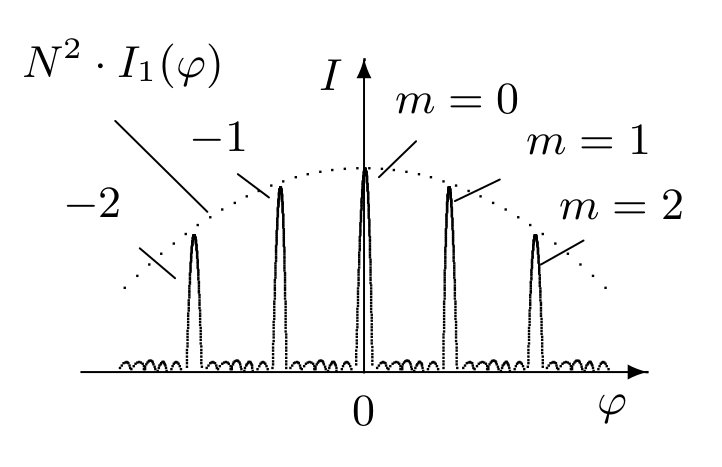
\includegraphics[width = 1.0\linewidth]{4.4.2/1.png}
    {Распределение интенсивности света при дифракции Фраунгофера на решётке}
\end{center}

Согласно принципу Гюйгенса-Френеля распределение интенсивности в дифракционной картине определяется суперпозицией волн; амплитуды всех интерферирующих волн при $\varphi$ практически одинаковы; фазы составляют арифметическую прогрессию:
\[
    d \sin \varphi_m = m \lambda,
 \]
 где $m \in Z$ "--- порядок спектра.
 
 Интенсивность $I$ света, распространяющегося под углом $\varphi$ к нормали:
 \[
 I = I_1(\varphi)\frac{\sin^2 (N(dk \sin \varphi) / 2)}{\sin^2 ((dk \sin \varphi) 2)},
 \]
 где $k = \frac{2 \pi}{\lambda}$ "--- волновое число.
 
 Дисперсия $D$ характеризует угловое расстояние между близкими спектральными линиями:
 \[
 D = \frac{d \varphi}{d \lambda} = \frac{m}{d \cos \varphi} = \frac{m}{\sqrt{d^2 - m^2 \lambda^2}}
 \]
 Согласно притерию разрешения Релея, линии становятся неразличимыми, когда расстояние между ними меньше, чем растояние от максимума одной линии до её первого минимума:
 \[
    \frac{Nkd}{2}(\sin (\varphi + \Delta \varphi) - \sin \varphi) = \pi,
 \]
 где $\Delta \varphi$ "--- угловая полуширина главного максимума, $\Delta \varphi = \frac{\lambda}{Nd \cos \varphi}$
 
 
 Разрешающая способность спектрального прибора $R$ вычисляется по формуле:
 \[
 R = \frac{\lambda}{\Delta \lambda} = m \cdot N
 \]
\begin{center}
    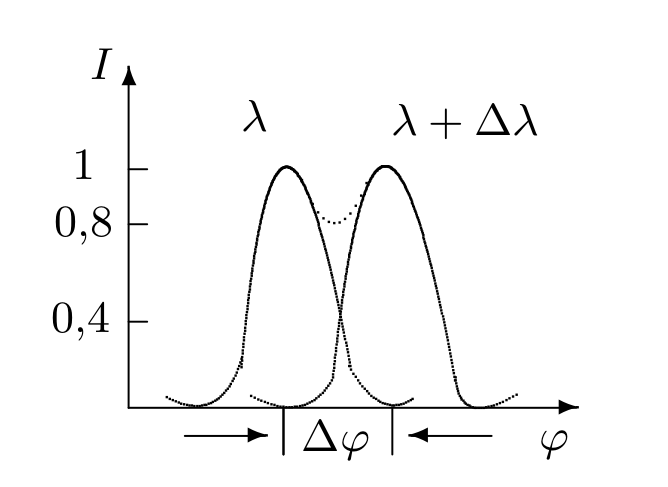
\includegraphics[width = 1.0\linewidth]{4.4.2/k.png}
    {К определению разрешающей способности дифракционной решётки}
\end{center}
Дисперсионная область $G$ "--- предельная ширина спектрального интервала $d \lambda$, при которой спектры соседних порядков перекрываются только своими границами:
\[
G = d \lambda = \frac{\lambda}{m}.
\]

\section*{Обработка результатов экспериментов}
При работе с дифракционной решёткой основной задачей является точное измерение углов, при которых наблюдается главные максимум для различных длин волн.
Эшелет "--- отражательная решётка с  треугольным профилем штриха, в которой угол $\Omega$ между рабочей гранью и плоскостью решётки не превышает $20^\circ$
Рабочий порядок $m \leq 10$, число штрихов $n = 1200\ штр/мм$.

Угол, под которым наблюдается максимум интенсивности функции $I_1 (\varphi)$, соответствует зеркальному отражению падающего луча от грани и называется углом блеска $\varphi_\text{б}$.
\[
    \varphi_\text{б} = \psi + 2 \Omega,
\]
где $\psi$ "--- угол, под которым падает плоская монохроматическая волна $\lambda$.

Разность хода $\Delta$ кратна $\lambda$:
\[
\Delta = d (\sin \varphi_m - \sin \varphi) = m \lambda.
\]
Изменяя угол падения, можно добиться того, чтобы угол блеска совпал с углом дифракции спектра одного из порядков; в этом порядке спектр будет наиболее ярким. Этот порядок принять называть рабочим.
\begin{center}
    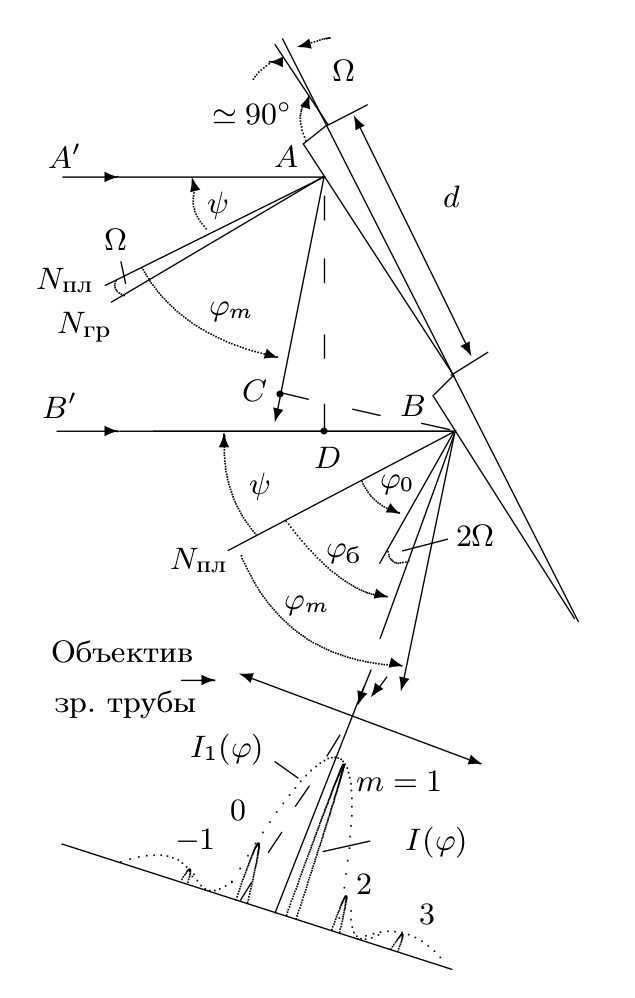
\includegraphics[width = 0.5\linewidth]{3.png} \\
    {Распределение интенсивности в спектре эшелета}
\end{center}

Чтобы устранить произвол в выборе угла падения, принято считать, что решётка должна работать в автоколлиматорном режиме. В этом случае условие $d(\sin \\varphi_m + \sin \varphi) = m \lambda$ принимает вид:
\[
    2d \sin \Omega = m_p \lambda_p.
\]
Для оценки $\Delta \varphi_m$ воспользуемся методом векторных диаграмм:
\begin{center}
    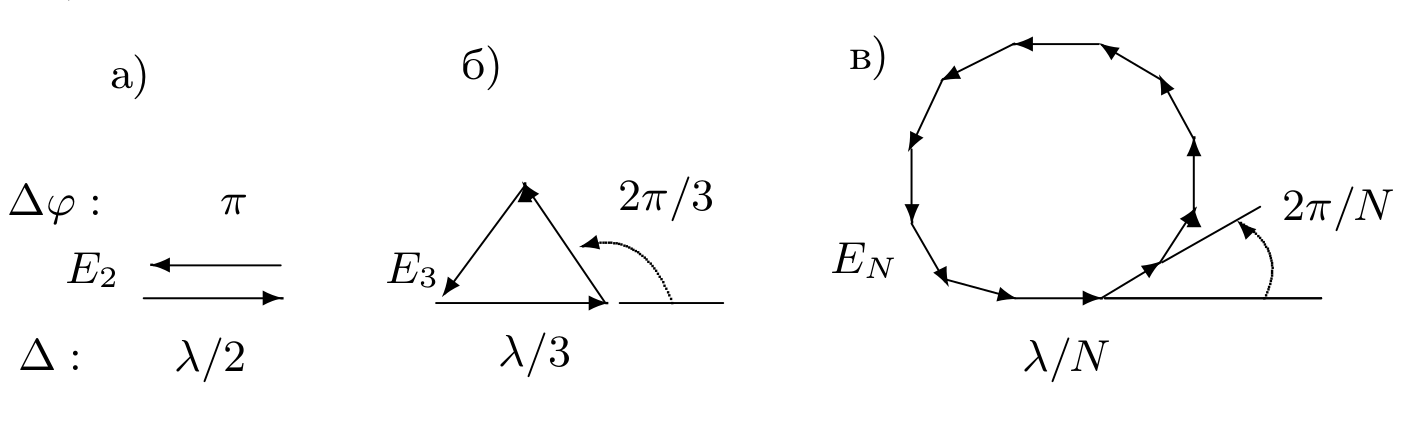
\includegraphics[width = 1.0\linewidth]{2.png}
    {Векторные диаграммы}
\end{center}
Направление на минимум, ближайший к максимуму любого порядка:
\[
d(\sin(\varphi_m + \Delta \varphi) + \sin \psi) = m \lambda + \frac{\lambda}{N}
\]
Для малой полуширины максимума получим:
\[
\Delta \varphi = \frac{\lambda}{Nd\cos \phi_m}
\]
Зависимость дисперсии $D$ от параметров эшелета:
\[
D = \frac{m}{d \cos \varphi_m} = \frac{m}{\sqrt{d^2 - (m \lambda - d \sin \psi)^2}}
\]

\section*{Результаты и обработка}
\subsection{1-17}
Произведём юстировку гониометра и установим начало отсчёта, руководствуясь техническим описанием.

Проделаем дополнительную настройку столика с эшелетом; установим $\psi = 30^\circ$; подберём ширину входной щели так, чтобы хорошо разрешались линии жёлтого дублета (ширина изображения щели чуть больше промежутка между линиями двойного штриха); установим высоту щели, удобную для измерений.

Для угла $\psi = 45^\circ$ измерим угловые координаты спектральных линий ртути в рабочем порядке. Отметим гловую координату каждой из описанных линий:\\
\begin{center}
\begin{tabular}{|c|c|c|}  \hline
Полоса         & $\varphi          $ & $\lambda, \dot A$ \\\hline
Фиолетовая     & $75^\circ 36' 45''$ & $4047$ \\\hline
Синяя          & $74^\circ 23' 45''$ & $4358$ \\\hline
Голубая        & $72^\circ 15' 35''$ & $4916$ \\\hline
Зелёная        & $70^\circ 12' 35''$ & $5461$ \\\hline
Желтая 2       & $69^\circ 3 ' 25''$ & $5770$ \\\hline
Жёлтая 1       & $68^\circ 58' 35''$ & $5791$ \\\hline
\end{tabular}
\end{center}

Для угла $\psi = 30^\circ$ измерим координаты каждой из жёлтых линий во всех наблюдаемых порядках:

\begin{center}
\begin{tabular}{|c|c|c|} \hline
& $Ж_1$ & $89^\circ3'55''$ \\
\cline{2-3}
$I_{пол}$
& $Ж_2$ & $88^055'45''$ \\\hline
& $Ж_1$ & $39^\circ50'55''$ \\
\cline{2-3}
$I_{отр}$
& $Ж_2$ & $39^\circ55'25''$ \\\hline
\end{tabular}
\end{center}
Повторим измерения для $\psi = 45^\circ, 60^\circ$:
   
\begin{center}
\begin{tabular}{|c|c|c|} \hline
& $Ж_1$ & $68^058'35''$\\
\cline{2-3}
$I_{отр}$
& $Ж_2$ & $69^\circ3'35''$ \\\hline
& $Ж_1$ & $48^\circ32'15''$ \\
\cline{2-3}
$II_{отр}$
& $Ж_2$ & $48^\circ40'50''$ \\\hline
\end{tabular}
$$\psi = 45^\circ$$
\end{center}
  
\begin{center}
\begin{tabular}{|c|c|c|} \hline
& $Ж_1$ & $92^\circ15'5''$\\
\cline{2-3}
$I_{отр}$
& $Ж_2$ & $92^\circ20'15''$ \\\hline
& $Ж_1$ & $70^\circ51'45''$ \\
\cline{2-3}
$II_{отр}$
& $Ж_2$ & $71^\circ0'35''$ \\\hline
& $Ж_1$ & $50^\circ51'5''$\\
\cline{2-3}
$III_{отр}$
& $Ж_2$ & $51^\circ4'45''$ \\\hline
\end{tabular}
$$\psi = 60^\circ$$
\end{center}

\textbf{Зависимость разрешающей силы от ширины пучка:}

Натроим зрительную трубу на желтый дублет в рабочем порядке; определим начало отсчёта "--- момент открытия щели. Крест появляется при $59^o57'20''$; ширина щели "--- 3 деления.

Откроем щель пошире; уменьшая ширину щели, добьемся предельного разрешения желтого дублета, оценим число штрихов:
\[
     n \approx 1600\ \text{штр}/\text{мм}; \quad \Delta \lambda = 2 \dot A.
\]
Построим график зависимости $\sin \varphi_m = f(\lambda)$ и по углу наклона определим период эшелета:

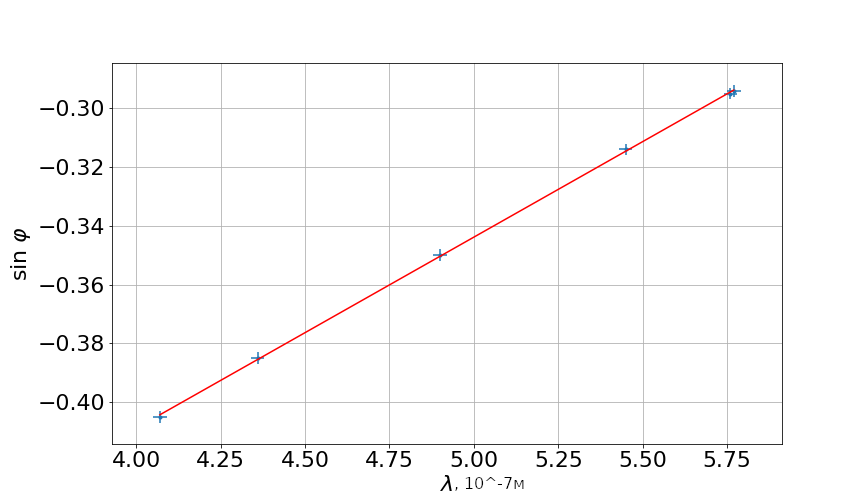
\includegraphics[width = 1.0\linewidth]{g1.png}
{Зависимость $\sin \varphi_m$ от $\lambda$}

Угол наклона графика $k = (6.5 \pm 0.1)\cdot 10^6 \text{м}^{-1}$

Число штрихов $n \approx 650 \pm 10\ \text{штр}/\text{мм}$

Период эшелета: $d = \frac{1}{0.65} = 1.53 \pm 0.04$ мм.

Угловая дисперсия в рабочем порядке для жёлтого дублета в угловых секундах на $\dot A$:
\[
D = 14.3\ \frac{\text{угл} \cdot \text{сек}}{\dot A}
\]
Экспериментальная разрешающая способность:
\[
R = \frac{\lambda}{\Delta \lambda} = 2890
\]

\section*{Вывод}
Мы научились работать с гониометром и измерили на немколичественно значения спектральных полос ртутной лампы с большой точностью.

\end{document}


125





\lipsum[1-4]
\begin{wrapfigure}{R}{5cm}
\centering
\includegraphics[width=0.20\textwidth]{rd.png}
\caption{1}
\end{wrapfigure}
\lipsum[1-6]


\begin{center}
\begin{center}$
\begin{array}{cccc}
\includegraphics[width=0.20\textwidth]{rd.png}&
\includegraphics[width=0.20\textwidth]{rd.png}&
\includegraphics[width=0.20\textwidth]{rd.png}&
\includegraphics[width=0.20\textwidth]{rd.png}\\
(1) & (2) & (3) & (4)
\end{array}$
\end{center}
\end{center}
